\subsection{График гистограммы распределения частот}

\FloatBarrier
\begin{figure}[h]
	\centering
	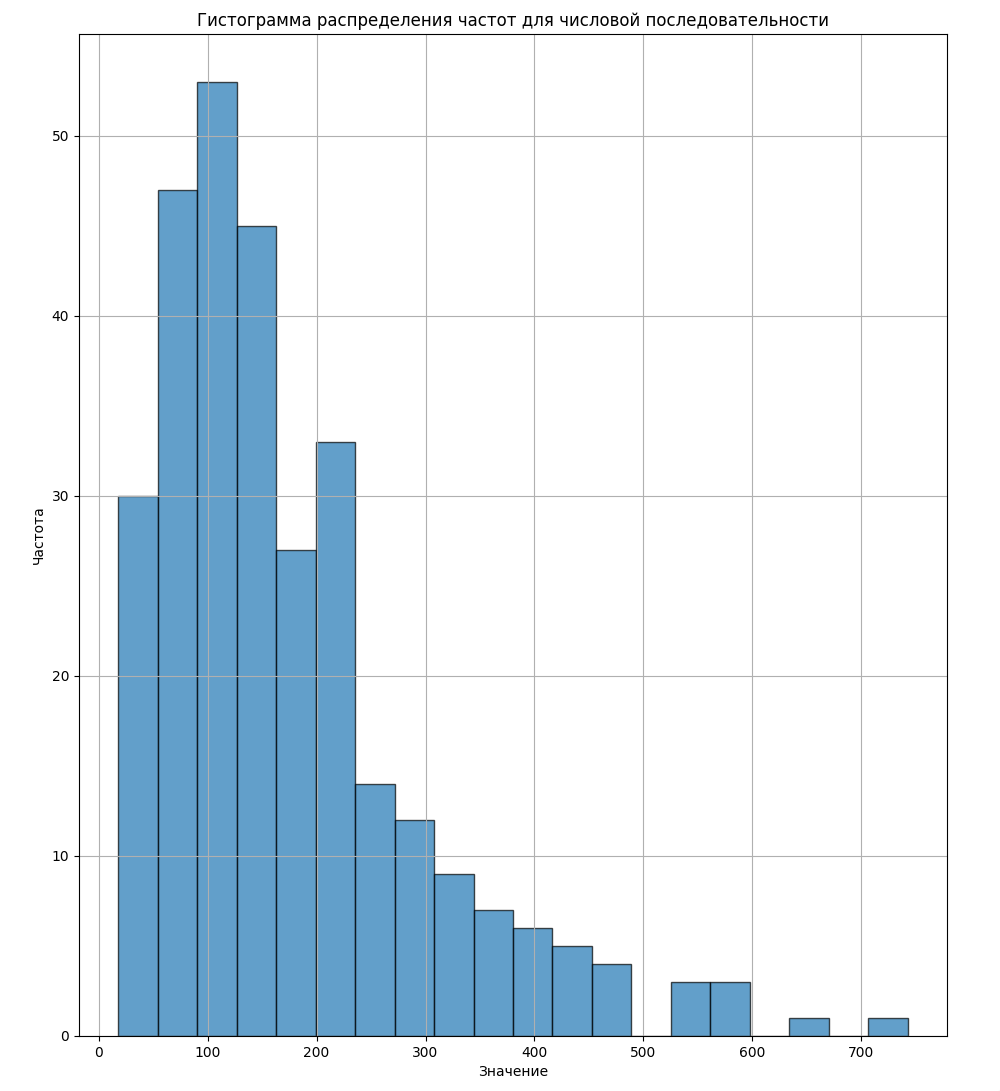
\includegraphics[width=0.7\textwidth]{../data/histogram.png}
	\caption{Гистограмма распределения частот заданной ЧП}
\end{figure}
\FloatBarrier

\subsection{Анализ и вывод}

Построенная гистограмма (рис. 1) представляет распределение частот для числовой последовательности. На графике можно заметить, что большинство значений сосредоточены в области с малыми числами, а частота встречаемости значений резко снижается по мере увеличения значений.

Такой характер распределения данных указывает на \textbf{экспоненциальное распределение}. Это видно из резкого спада частоты по мере увеличения величины, что является характерной чертой экспоненциального распределения.
